% $Header$

\documentclass{beamer}
\usepackage{tikz-cd}
\usepackage{amscd}
\usepackage{tikz-cd}
\usepackage{dsfont}
\usepackage{comment}
\newtheorem{conjecture}{Conjecture}
\newtheorem{conjeorem}{Conjeorem}
\usepackage{mathabx,epsfig}
\usepackage{tcolorbox}
\usepackage[document]{ragged2e}
\def\acts{\mathrel{\reflectbox{$\righttoleftarrow$}}}

\newcommand*\circled[1]{\tikz[baseline=(char.base)]{        \node[shape=circle,draw,inner sep=0.8pt] (char) {#1};}}

\mode<presentation>
{
  \usetheme{Boadilla}
  % or ...

  \setbeamercovered{invisible}
  % or whatever (possibly just delete it)
}

\setbeamertemplate{navigation symbols}{}
\setbeamertemplate{page number in head/foot}{}


\usepackage[english]{babel}
% or whatever

\usepackage[latin1]{inputenc}
% or whatever

\usepackage{times}
\usepackage[T1]{fontenc}
% Or whatever. Note that the encoding and the font should match. If T1
% does not look nice, try deleting the line with the fontenc.


\title[] % (optional, use only with long paper titles)
{Homotopically Standard Tight Non-fillable Contact Structures on the Sphere}

\subtitle
{}

\author[Josua Kugler] % (optional, use only with lots of authors)
{Josua Kugler \texorpdfstring{\\}{} results by Bowden, Gironella, Moreno and Zhou}

% - Give the names in the same order as the appear in the paper.
% - Use the \inst{?} command only if the authors have different
%   affiliation.

\institute% (optional, but mostly needed)
{Heidelberg University}
% - Use the \inst command only if there are several affiliations.
% - Keep it simple, no one is interested in your street address.

\date[Sep 17th 2024] % (optional, should be abbreviation of conference name)
% - Either use conference name or its abbreviation.
% - Not really informative to the audience, more for people (including
%   yourself) who are reading the slides online

\subject{Symplectic and Contact Topology}
% This is only inserted into the PDF information catalog. Can be left
% out. 



% If you have a file called "university-logo-filename.xxx", where xxx
% is a graphic format that can be processed by latex or pdflatex,
% resp., then you can add a logo as follows:

% \pgfdeclareimage[height=0.5cm]{university-logo}{university-logo-filename}
% \logo{\pgfuseimage{university-logo}}



% Delete this, if you do not want the table of contents to pop up at
% the beginning of each subsection:
%\AtBeginSubsection[]
%{
 % \begin{frame}<beamer>{Outline}
  %  \tableofcontents[currentsection,currentsubsection]
  %\end{frame}
%}


% If you wish to uncover everything in a step-wise fashion, uncomment
% the following command: 

%\beamerdefaultoverlayspecification{<+->}

\makeatletter
    \newenvironment{withoutheadline}{
        \setbeamertemplate{headline}[default]
        \def\beamer@entrycode{\vspace*{-\headheight}}
    }{}
\makeatother

\begin{document}

\begin{frame}
  \titlepage
\end{frame}


% Structuring a talk is a difficult task and the following structure
% may not be suitable. Here are some rules that apply for this
% solution: 

% - Exactly two or three sections (other than the summary).
% - At *most* three subsections per section.
% - Talk about 30s to 2min per frame. So there should be between about
%   15 and 30 frames, all told.

% - A conference audience is likely to know very little of what you
%   are going to talk about. So *simplify*!
% - In a 20min talk, getting the main ideas across is hard
%   enough. Leave out details, even if it means being less precise than
%   you think necessary.
% - If you omit details that are vital to the proof/implementation,
%   just say so once. Everybody will be happy with that.

%\begin{frame}{Contact geometry and Reeb dynamics}

%A contact manifold is $(M^{2n+1},\xi=\ker \alpha)$, where $\alpha\wedge d\alpha^n>0$, $\alpha$ the contact $1$-form.

%\begin{center}
%\mbox{The Reeb field is} $R_\alpha: \;d\alpha(R_\alpha,\cdot)=0,\; \alpha(R_\alpha)=1.$  
%\end{center}

%\pause

%\begin{conjecture}[Weinstein] Every Reeb dynamics admits at least one periodic orbit. 
%\end{conjecture}

%\pause

%\begin{exampleblock}{}
%\begin{center}
%Geometry $\longleftrightarrow$  Dynamics
%\end{center}
%\end{exampleblock}

%Proved by Taubes in dimension $3$, open in higher dimension.
    
%\end{frame}

\begin{frame}
\begin{tcolorbox}
\Huge \begin{center}
    \textbf{Background}
\end{center}
\end{tcolorbox}
\end{frame}

\begin{frame}{Contact topology}

\textbf{Contact topology:} The study of contact manifolds, up to isotopy.

\medskip

\pause

\textbf{Fillability:} \emph{fillable} contact mflds are boundaries of symplectic mflds.

\pause

\begin{exampleblock}{Fillability question}  Which contact manifolds are \textbf{fillable}?
\end{exampleblock}

\pause

Eliashberg, Borman--Eliashberg--Murphy:

\begin{tcolorbox}
\textbf{Dichotomy:} Rigidity vs.\ Flexibility. 
\begin{itemize}
    \item \textbf{tight} \emph{(rigid/geometric)};
    \item  \textbf{overtwisted} \emph{(flexible/topological)}. 
\end{itemize}
\end{tcolorbox} 

\pause

\begin{theorem}[Eliashberg--Gromov]
Fillable contact manifolds are tight.
\end{theorem}

Converse is false (Etnyre--Honda, Massot--Niederkrueger--Wendl).

\end{frame}

\begin{frame}{Existence and classification}

\emph{Topological} obstruction: \emph{almost} contact structure, i.e.\ reduction of structure group to $U(n)\times \mathds 1$.

\begin{theorem}[Lutz--Martinet (dim 3), Casals--Pancholi--Presas (dim 5), Borman--Eliashberg--Murphy (any dim)]

Almost contact manifolds are contact, where the contact structure is \emph{overtwisted}.

\end{theorem}

\pause

\begin{exampleblock}{Tight manifolds}
How can we understand \textbf{tight} contact manifolds?
\end{exampleblock}
    
\end{frame}

\begin{frame}{Contact topology: fillability}

\begin{tcolorbox} \textbf{Hierarchy of fillability:}
$$\{Stein\}\stackrel{\circled{1}}{=}\{Weinstein\}\stackrel{\circled{2}}{\subsetneq} \{Liouville\}\stackrel{\circled{3}}{\subsetneq} \{strong\}$$
$$\stackrel{\circled{4}}{\subsetneq}\{weak\}
\stackrel{\circled{5}}{\subsetneq} \{tight\}$$
\end{tcolorbox} 

$\bullet \;dim=3$: \circled{1} Cieliebak--Eliashberg, \circled{2} Bowden, \circled{3} Ghiggini, \circled{4} Eliashberg, \circled{5} Etnyre--Honda.

\medskip

$\bullet \;dim \geq 5$: \circled{1} Cieliebak--Eliashberg, 

\circled{2} Bowden--Crowley--Stipsicz, \circled{3} Zhou, 

\circled{4} Bowden--Gironella--M., \circled{5} Massot--Niederkr\"uger--Wendl. 

\end{frame}

\begin{frame}{Contact structures on spheres}

\textbf{First step in classification:} contact structures on spheres.

\begin{exampleblock}{Standard contact structure}
The standard contact structure is $(S^{2n-1},\xi)=\partial(B^{2n},\omega_{std})$.
\end{exampleblock}

\pause

\begin{theorem}[Eliashberg, '91] 
    On $S^3$, it is the unique tight contact structure.
\end{theorem} 

In particular, no tight and non-fillable contact structures on $S^3$.

    %\item Eliashberg ('91): $n\geq 2$, $S^{2n+1}$ has non-standard fillable  structures.
    %\item Ustilovsky ('99): $n\geq 2$, $S^{4n+1}$, infinitely many structures.
    %\item Ding--Geiges ('04): every odd sphere has non-standard contact structures.
    
    
    %\medskip
    
    %Uebele ('16), Alves--Meiwes ('19, dynamical properties), Lazarev ('20, flexible fillings),...
    


\end{frame}

\begin{frame}{Tight and non-fillable structures in $\dim \geq 5$}

\begin{theorem}[Bowden--Gironella--M.--Zhou '22-'24]
In $\dim \geq 7$, if $M$ admits a tight structure, it also admits a tight and non strongly-fillable structure, in the same almost contact class. 
\pause

\smallskip

In $\dim=5$, the same holds, if the first Chern class vanishes.
\end{theorem}

%I.e.\ the classical topology (and almost contact class) are \emph{standard}. \pause By taking a contact connected sum with a non-standard sphere:

We get infinitely many if $\dim \geq 11$, and $M$ is Weinstein fillable with torsion first Chern class.

    
\end{frame}

\begin{frame}{Case of spheres}

The general theorem follows by connected sum with an ``exotic'' sphere:

\begin{theorem}[Bowden--Gironella--M.--Zhou '22-'24]
    For every $n \geq 2$, the sphere $\mathbb S^{2n+1}$ admits a tight, non-fillable contact structure that is homotopically standard.
\end{theorem}

\pause

Infinitely many if $n\geq 5$.
    
\end{frame}

\begin{frame}{General remarks}

\begin{itemize}
    \item This is a novel and strictly higher-dimensional phenomenon (false in dim $3$).

\pause
    
    \item Suggests that higher-dimensional contact phenomena should occur independently of underlying smooth topology.
\end{itemize}

    
\end{frame}

\begin{frame}{Liouville but not Weinstein}

\begin{theorem}[Bowden--Gironella--M.--Zhou '22-'24]
    In $\dim \geq 7$, if $M$ admits a Weinstein fillable structure with torsion first Chern class, then it also admits infinitely many Liouville but non-Weinstein fillable structures in the same formal class.
\end{theorem}
    
\end{frame}

\begin{frame}{Case of spheres}

This again follows by connected sum with an ''exotic'' sphere:

\begin{theorem}[Bowden--Gironella--M.--Zhou '22]
For any $n \ge 3$, there exist infinitely many Liouville fillable contact structures on $\mathbb S^{2n+1}$ that are not Weinstein fillable, and are homotopically standard.
\end{theorem}
    
\end{frame}

\begin{frame}

\begin{exampleblock}{Open questions}
\begin{itemize}
    \item Is there a Liouville but not Weinstein fillable structure on $\mathbb S^5$?
    \item Is there a strong but not Liouville fillable structure on $\mathbb S^{2n+1},$ $n\geq 2$?
\end{itemize}

\end{exampleblock}
 
\end{frame}

\begin{frame}
\begin{tcolorbox}
\Huge \begin{center}
    \textbf{Tight and non-fillable spheres}
\end{center}
\end{tcolorbox}
\end{frame}

\begin{frame}{Giroux correspondence}

\begin{tcolorbox}
\textbf{Giroux:} Contact structures are \emph{supported} by open books.
\end{tcolorbox} 

\begin{figure}
    \centering
    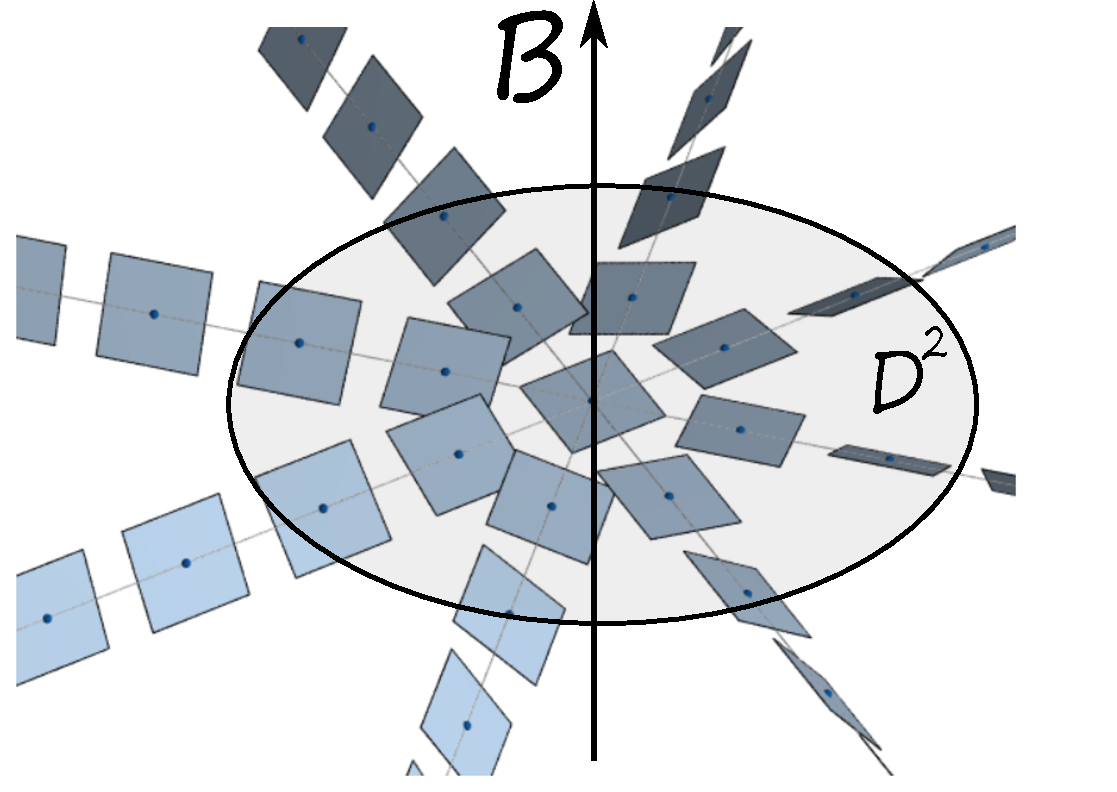
\includegraphics[width=0.6\linewidth]{standardctct.pdf}
    \caption{Supported contact structure.}
    \label{fig:adapted}
\end{figure}

\end{frame}

\begin{frame}{Bourgeois contact structures}
    \begin{theorem}[Bourgeois '02]
    Open book supporting $(M,\xi)\rightsquigarrow$ contact structure on $M\times \mathbb T^2$.
    \end{theorem}

 These are $\mathbb T^2$-equivariant.   
    
\end{frame}

\begin{frame}{Geometric construction}
    
    \textbf{Geometric construction:} We now construct \textbf{one} tight and non-fillable contact structure on $\mathbb S^{2n+1}$.
    
    \medskip
    
    \pause

    \begin{itemize}
        \item Milnor open book on $\mathbb S^{2n-1}\rightsquigarrow$ Bourgeois manifold on $\mathbb S^{2n-1}\times \mathbb T^2$
    $\rightsquigarrow $ two $1$-surgeries = $\mathbb S^{2n-1}\times \mathbb S^2 \rightsquigarrow$ one $2$-surgery = $\mathbb S^{2n+1}.$
    
    \medskip

    \pause
    
    \item If $n\geq 3,$ surgeries are \emph{subcritical} $\rightsquigarrow$ by 'Eliashberg's' h-pple, Weinstein cobordism $\rightsquigarrow$ contact manifold $(\mathbb S^{2n+1},\xi_{ex})$.

    \end{itemize}

    \pause
    
    \medskip

    \begin{tcolorbox}
    \textbf{Claim:} $(\mathbb S^{2n+1},\xi_{ex})$ is tight and non-fillable.
    \end{tcolorbox}
    
\end{frame}

\begin{frame}{Tightness and fillability from algebraic perspective}

Contact homology algebra $CHA(Y)$ (homology well-defined by Pardon).

\begin{definition}

\begin{enumerate}
    \item $Y$ is \emph{algebraically} tight if $CHA(Y)\neq 0$.
    \item $Y$ is \emph{algebraically} fillable if there is a DGA augmentation of $CHA(Y)$ at the chain level.
\end{enumerate} 
Similarly for \emph{algebraically} overtwisted/non-fillable.
\end{definition}

\textbf{Note:} This definition is well-defined, due to functoriality of the DGA, even though homotopy type of chain level is not.
\end{frame}

\begin{frame}{Formal algebraic properties}

\begin{lemma}
    \begin{enumerate}
        \item Algebraically tight $\Rightarrow$ tight.
        \item Algebraically fillable $\Rightarrow$ algebraically tight.
        \item Algebraically non-fillable $\Rightarrow$ non-fillable.
        \item $1$-ADC $\Rightarrow$ algebraically tight.
    \end{enumerate}
\end{lemma}

$1$-ADC is an \emph{index-positivity} condition (Lazarev, Zhou).

%there exists a decreasing sequence of contact forms so that contractible orbits below an action window (going to infinity) have \emph{degree} less than 1. 

\medskip

\pause

\textbf{Facts:} \begin{enumerate}
    \item (Advek '22) tight contact manifolds can be algebraically overtwisted, in dim 3.
    \item Algebraic tightness is preserved under surgeries. Tightness is also, in dim $3$ (Wand '14).
    \item $1$-ADC binding of fillable open book $\Rightarrow$ $1$-ADC algebraically fillable Bourgeois manifold $\Rightarrow$ algebraically tight. 
    \item E.g.\ Milnor $A_k$-singularity open book has $1$-ADC binding.
\end{enumerate}

\end{frame}

\begin{frame}{Tightness}

\begin{tcolorbox}
Milnor $A_k$ open book $\Rightarrow (\mathbb S^{2n+1},\xi_{ex})$ is \emph{tight}.
\end{tcolorbox}

\pause

\begin{tcolorbox}
\textbf{Note:} Heuristically, there is a priori \emph{many} choices of open book. This suggests \emph{many} non-standard structures. However, distinguishing is subtle.
\end{tcolorbox}

\end{frame}

\begin{frame}{Non-fillability}

\textbf{Non-fillability} of $(\mathbb S^{2n+1},\xi_{ex})$ can be proven via:

\begin{enumerate}
    \item Homological obstruction and cobordisms as in [Bowden--Gironella--M.], building on [Massot--Niederkr\"uger--Wendl].
    \item Symplectic cohomology computations as in [Zhou].
\end{enumerate}

\end{frame}

\begin{frame}{Homological obstructions}

\textbf{Observation:} Bourgeois manifolds have convex decomposition $$M\times \mathbb T^2=(M\times \mathbb S^1)\times \mathbb S^1= V_+\times \mathbb S^1 \cup_\phi \overline{V}_-\times \mathbb S^1,$$ with $V_\pm=\Sigma \times D^*\mathbb S^1$, $\Sigma=$ page of the open book, $\phi=$ monodromy.

\pause

\begin{theorem}[Bowden--Gironella--M.]

$M=V\times \mathbb S^1=V_+\times \mathbb S^1\cup_\phi \overline{V_-}\times \mathbb S^1$ with convex decomposition, $N=\partial V_\pm$ dividing set. If $W$ is a symplectic filling of $M$, then
$$
H_*(N)\rightarrow H_*(V_\pm) \rightarrow H_*(W),
$$
induced by inclusion. Then second map is injective on image of the first.
\end{theorem}

Namely, if a homology class in $N$ survives in $V_\pm$, then it survives in the filling.
    
\end{frame}

\begin{frame}{Idea of proof}

\begin{itemize}
\item Capping cobordism from $M$ to $N\times \mathbb S^2$ with a SHS, via handles $H_\pm$ with co-core $V_\pm$. 

\pause

\item Second factor gives moduli space of spheres $\mathcal M_*$ with evaluation map $ev: \mathcal M_*\rightarrow W$. 

\pause

\item Spheres intersect $H_\pm$ precisely once $\rightsquigarrow$ intersection map $\mathcal I_\pm:\mathcal M_*\rightarrow V_\pm$.

\pause

\item If $\sigma \subset W$ satisfies $\partial \sigma=c$ with $c$ cycle in $N$, then $b=\mathcal I_\pm ev^{-1}(\sigma)$ bounds $\sigma$ in $V_\pm$. $\hfill\square$ 

\end{itemize}
    
\end{frame}

\begin{frame}{Homological obstructions}

\textbf{Fact:} 

\begin{enumerate}
    \item If $\dim \geq 7$, subcritical surgeries on $\mathbb S^{2n-1}\times \mathbb T^2$ can be pushed away from dividing set to $V_+$.
$$
\Rightarrow (\mathbb S^{2n+1},\xi_{ex}) \mbox{ still has a dividing set } N,
$$
with $H_n(N)\neq 0$.

\pause 
\item Homological obstruction theorem persists under surgery away from dividing set (capping cobordisms).
\end{enumerate}


\begin{figure}
    \centering
    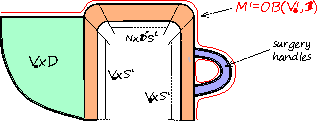
\includegraphics[width=0.7\linewidth]{blowdown_handle.pdf}
    \caption{Capping cobordism.}
    \label{fig:capping_cobordism}
\end{figure}

\end{frame}

\begin{frame}

\textbf{End of the proof:} $W$ filling of $(\mathbb S^{2n+1},\xi_{ex}) \Rightarrow$ Homological obstruction: 

$$
0\neq H_n(N) \hookrightarrow H_n(W).
$$
However, this factors as
$$
0\neq H_n(N) \rightarrow H_n(\mathbb S^{2n+1})=0 \rightarrow H_n(W),
$$
contradiction.
\end{frame}

\begin{frame}{Remarks}

\begin{enumerate}
    \item \textbf{Homotopically standard:} Fixed $\xi$, Bourgeois manifolds have same almost contact class $\xi \oplus T\mathbb T^2$, so suffices with trivial open book. $h$-cobordism theorem gives standard smooth topology on sphere.

\pause

    \item \textbf{Infinitely many:} connected sums with Lazarev's non-standard flexibly fillable spheres. Distinguished by positive symplectic cohomology (Cieliebak--Oancea).

\pause
    
    \item \textbf{Dimension $5$:} Needs careful \emph{flexible} version of the homological obstruction theorem.

    \pause
    
    \item \textbf{Symplectic cohomology:} Capping cobordisms reach $\partial(V\times \mathbb D^2)$. Zhou's computations of $SH_+(\partial(V\times \mathbb D^2))$ and $SH_+$ computations of Brieskorn spheres as by [Kwon--van-Koert] can be used.  
    
\end{enumerate}
    
\end{frame}

\begin{frame}
\begin{tcolorbox}
\Huge \begin{center}
    \textbf{Liouville but not Weinstein fillable spheres}
\end{center}
\end{tcolorbox}
\end{frame}

\begin{frame}{Geometric construction}
    \textbf{One} example: 

    \medskip

    \begin{itemize}
    
    \item $V=N^{2n-1}\times [-1,1]$ Liouville domain (MNW) $\rightsquigarrow$ $M=\partial (V \times \mathbb D^2)$, which is ADC (Lazarev, Zhou). 

    \medskip

    \pause
    
    \item Bowden--Crowley--Stipsicz  $\rightsquigarrow$ cobordism $W$ to sphere $\mathbb S^{2n+1}$.

    \medskip

    \pause

    \item Cieliebak--Eliashberg  $\rightsquigarrow$ $W$ can be taken flexible Weinstein $\rightsquigarrow$ contact sphere $(\mathbb S^{2n+1},\xi)$, which is ADC.

    \medskip

    \pause

    \item Stacking $W$ on top of $V\times \mathbb D^2$ $\rightsquigarrow$ $(\mathbb S^{2n+1},\xi)$ has Liouville filling $X^{2n+2}=V\times \mathbb D^2\cup W$. 

\end{itemize}

    \medskip 

    \pause
    
\begin{exampleblock}{}
    \textbf{Note:} $H_{2n-1}(X)\neq 0$, coming from $[N]$, and $2n-1>n+1$ if $n\geq 3$ $\Rightarrow X$ \textbf{not} Weinstein (if $n=2$, it is by Breen--Christian).
\end{exampleblock}

    \pause

     \medskip 

    $X'$ another filling, ADC $\rightsquigarrow$ $H_*(W)\cong H_*(W')$ (Zhou) $\Rightarrow$ \textbf{not} Weinstein fillable. 
\end{frame}

\begin{frame}
\centering
Thank you!
    
\end{frame}

\end{document}